% Chapter Template

\chapter{Results} % Main chapter title

\label{Chapter3} % Change 3 to a consecutive number; for referencing this chapter elsewhere, use \ref{Chapter3}

\lhead{\emph{Results}} % Change X to a consecutive number; this is for the header on each page - perhaps a shortened title

%----------------------------------------------------------------------------------------
%   SECTION 1
%----------------------------------------------------------------------------------------

\section{Ternary Diagrams}

Using the methods described in Section \ref{Chapter2}, Ternary phase diagrams for each of the four combinations of elements at 298K were produced and reduced - these diagrams are present in \ref{fig:298KTPD}. 

\begin{figure}[ht]
\centering
\begin{subfigure}{70mm}
  \centering
    \includegraphics[width=70mm]{triangleplot_CUZNS298.png}
    \caption{Cu, Zn, S Ternary Diagram}
    \label{fig:CuZnS}
\end{subfigure}%
\begin{subfigure}{70mm}
 \centering
    \includegraphics[width=70mm]{triangleplot_CUZNSN298.png}
    \caption{Cu, Zn, Sn Ternary Diagram}
    \label{fig:CuZnSn}
\end{subfigure}
\begin{subfigure}{70mm}
 \centering
    \includegraphics[width=70mm]{triangleplot_CUSNS298.png}
    \caption{Cu, Sn, S Ternary Diagram}
    \label{fig:CuSnS}
\end{subfigure}
\begin{subfigure}{70mm}
 \centering
    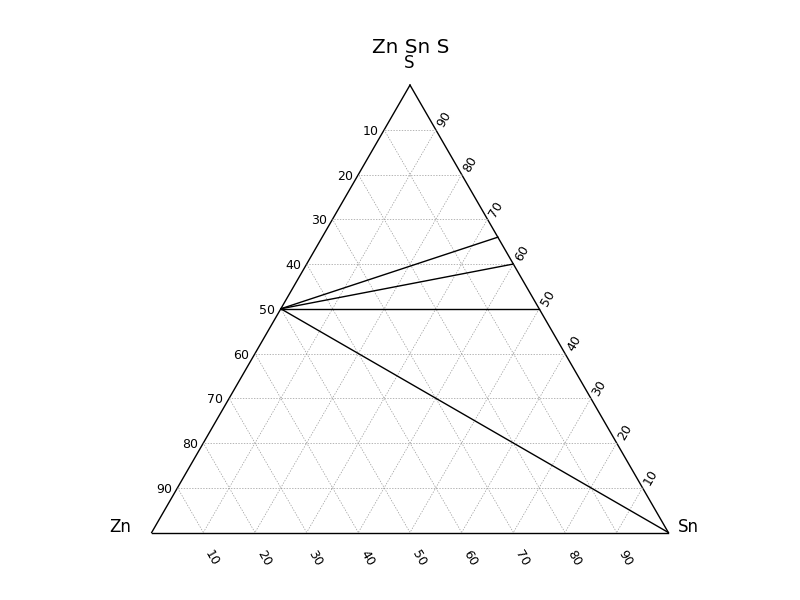
\includegraphics[width=70mm]{triangleplot_ZnSnS298.png}
    \caption{Zn, Sn,S Ternary Diagram}
    \label{fig:ZnSnS}
\end{subfigure}
\caption{Ternary Diagrams of the remaining face, post Tie-line calculations.}
\label{fig:298KTPD}
\end{figure}

%----------------------------------------------------------------------------------------
%   SUBSECTION 1
%----------------------------------------------------------------------------------------

\subsection{Quaternary Diagram}

A quaternary phase diagram was produced by joining the Ternary phase Diagrams along their common edges, and the tie-phases examined. A model of this is presented in \ref{AppendixC}, and a simplified model flattened in the z-axis, with the Cu-Zn-Sn Ternary Phase diagram omitted is presented in \ref{fig:298KQPD}. This diagram effectively presents the sets of tie-lines situated closely to sulphur which join together to form five candidate quasi-ternary phases, whose compositions are as follows: ZnS-SnS-Cu, ZnS-SnS-Cu$_2$S, ZnS-Sn$_2$S$_3$-Cu$_2$S, ZnS-SnS$_2$-Cu$_2$S, ZnS-SnS$_2$-CuS. Each tie-phase was examined to determine whether it held the correct ratio of elements to form CZTS, initially starting with ensuring a 1:1 ratio of Sulphur to the rest of the elements combined. This yielded 2 possible candidates from the group of tie-phases. Subsequently, these two candidates were examined to determine whether they held a composition ratio of 2:1:1 of Cu, Zn and Sn; of the two only one had the correct composition ratio: ZnS-SnS$_2$-Cu$_2$S.


\begin{figure}[ht]
\centering
    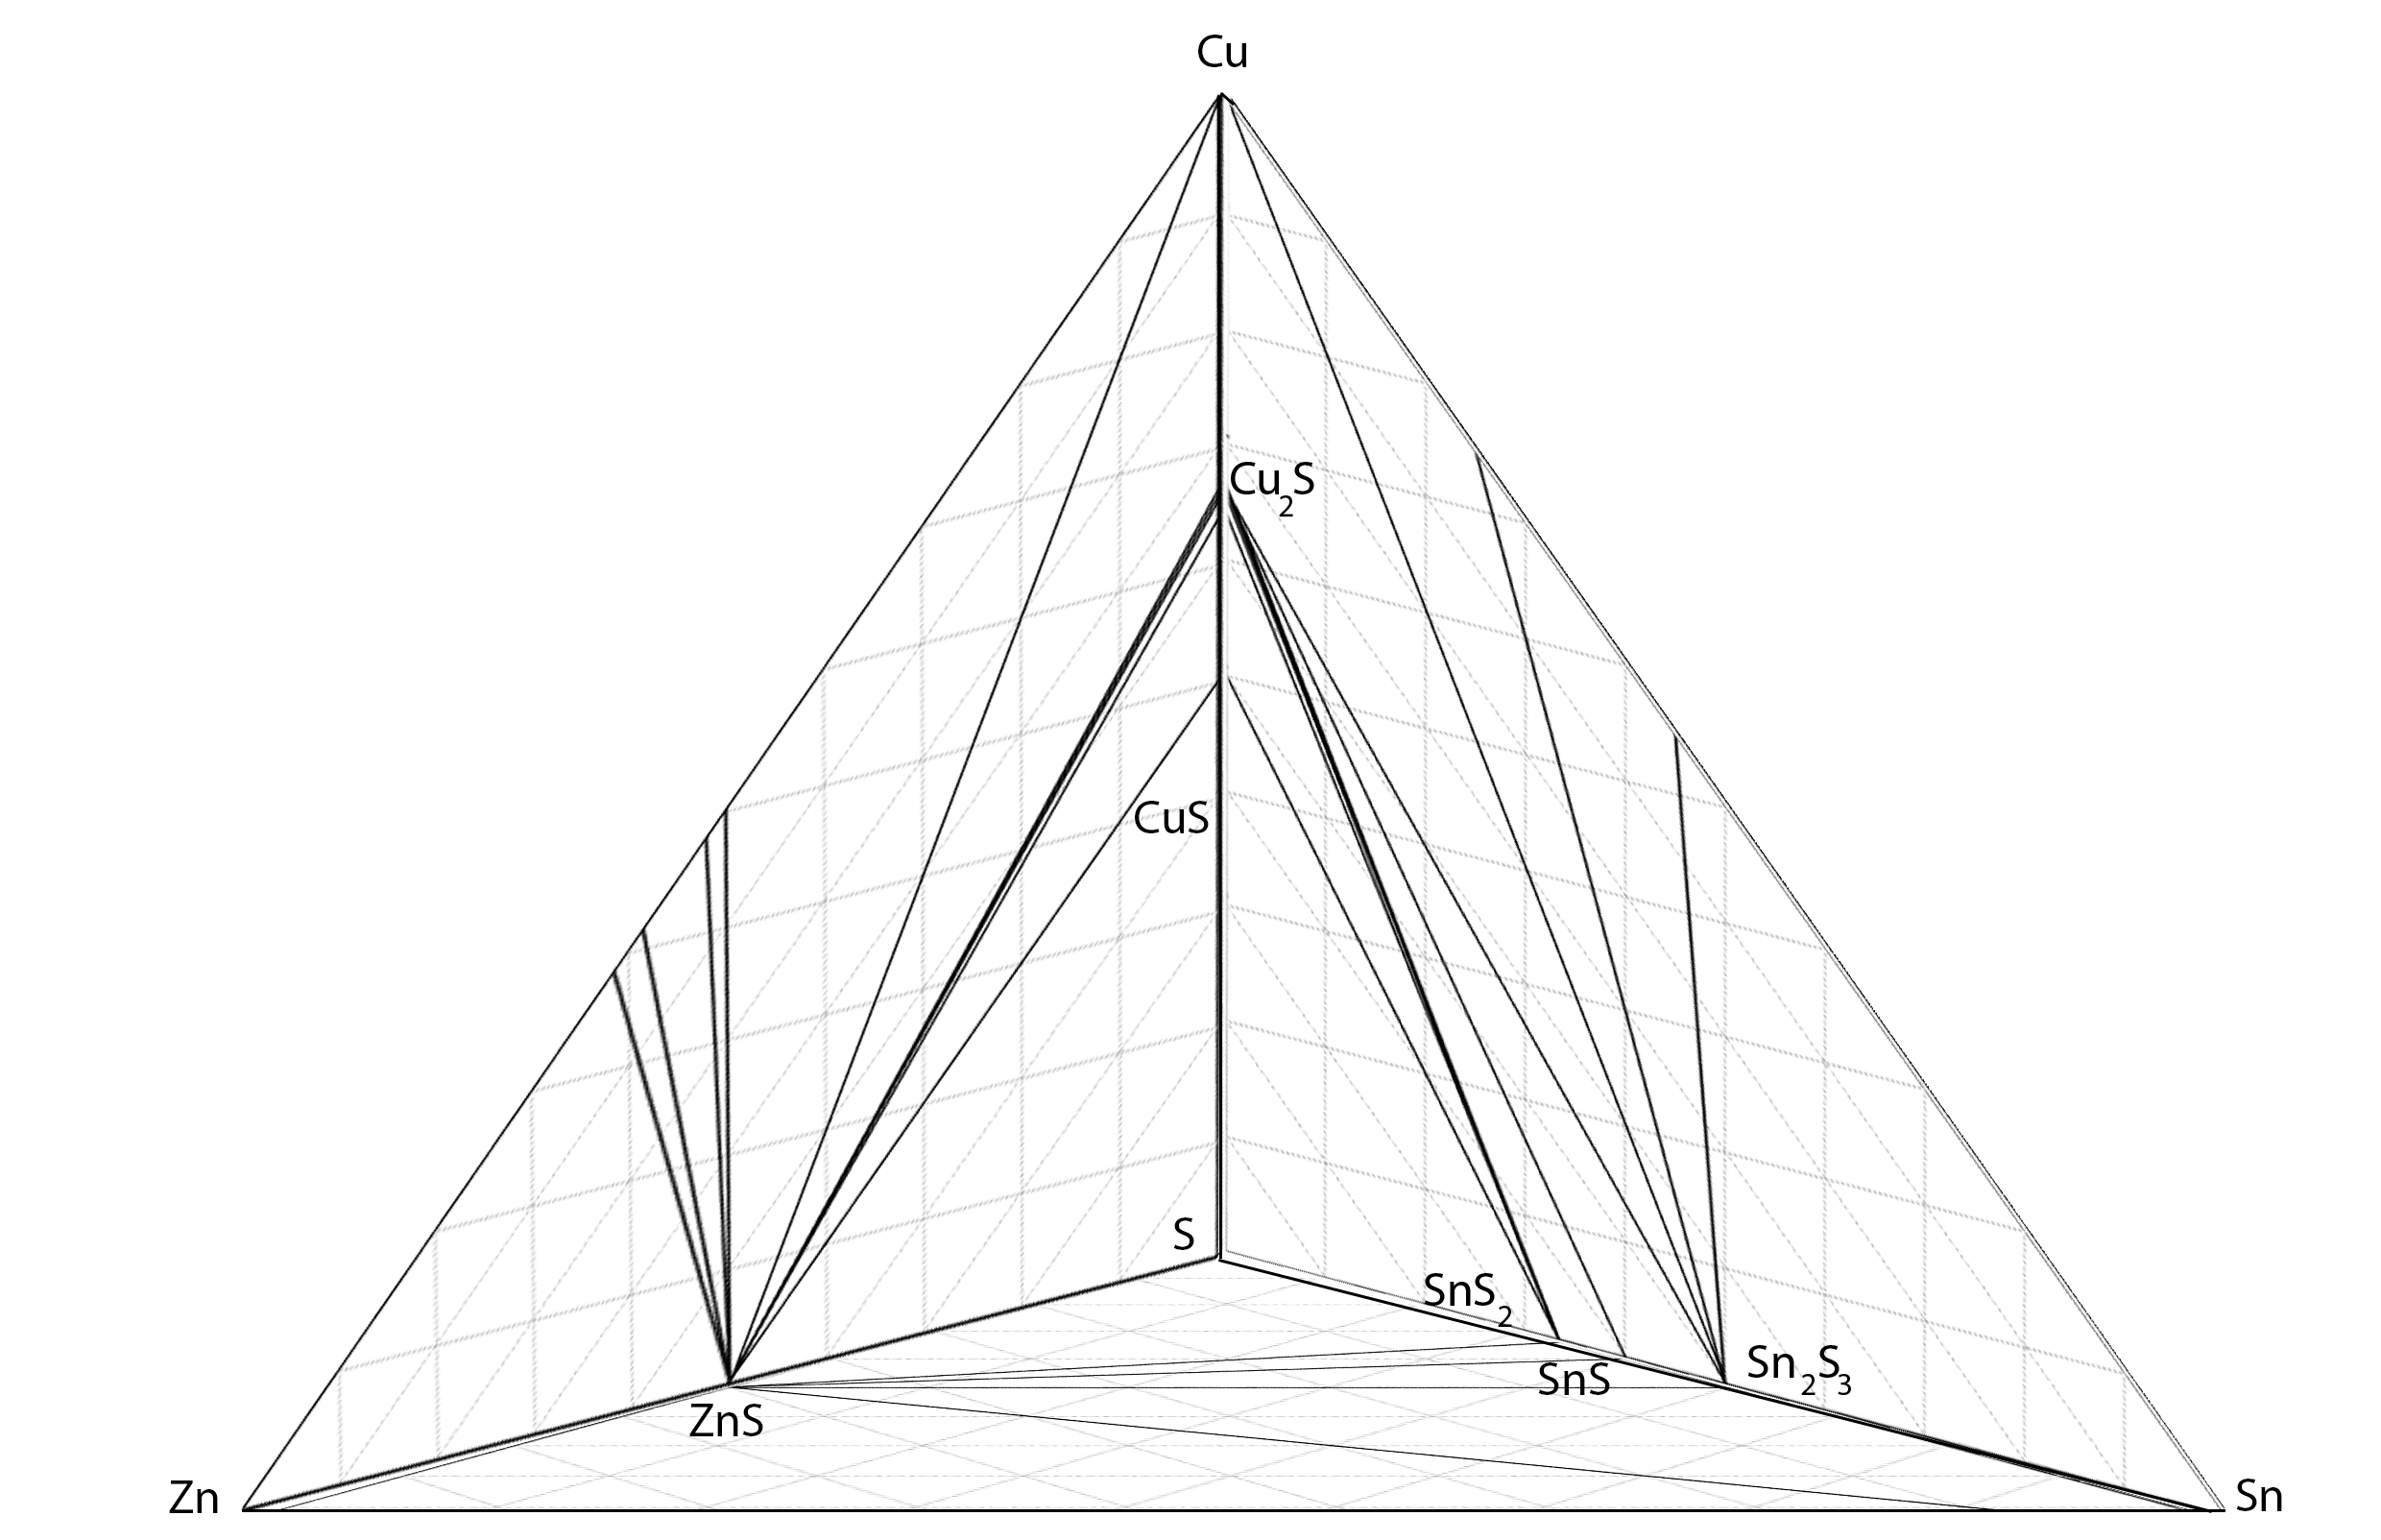
\includegraphics[width=130mm]{FlatQPD.png}
    \caption{Simplified Quaternary Phase Diagram, Omitting the CuZnSn Ternary Phase with the 'corners' of the tie-phases labelled.}
\label{fig:298KQPD}
\end{figure}
%----------------------------------------------------------------------------------------
%   SECTION 2
%----------------------------------------------------------------------------------------

\section{Quasi-Ternary Diagrams}


\begin{figure}
\centering
 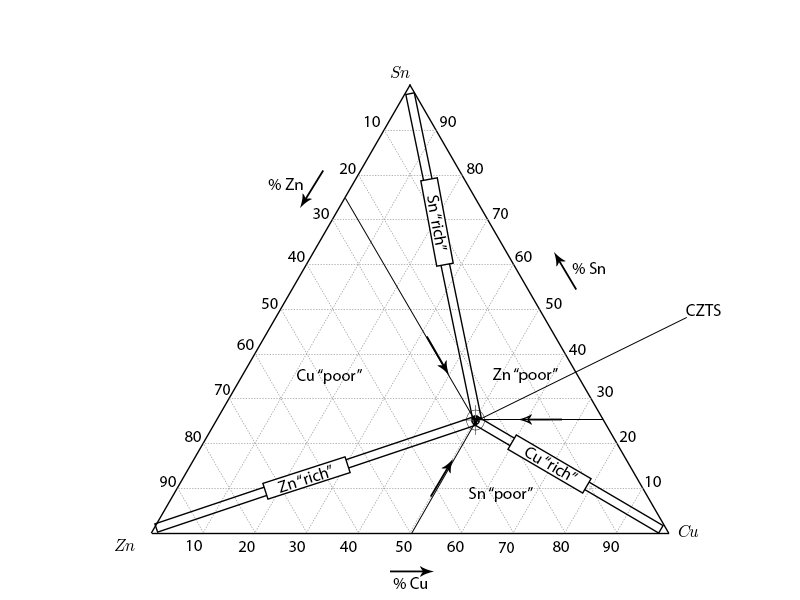
\includegraphics[width=130mm]{ZnSSn2S3Cu2S-general}
    \caption{Location of CZTS, and labelled secondary phases.}
    \label{fig:ZnSSn2S3Cu2S}
\end{figure}
